%=======================02-713 LaTeX template, following the 15-210 template==================
%
% You don't need to this template
%
\documentclass[11pt]{article}
\usepackage{amsmath,amssymb,amsthm}
\usepackage{graphicx}
\usepackage[margin=1in]{geometry}
\usepackage{fancyhdr}
\setlength{\parindent}{0pt}
\setlength{\parskip}{5pt plus 1pt}
\setlength{\headheight}{13.6pt}
\newcommand\tab[1][1cm]{\hspace*{#1}}
\newcommand\question[2]{\vspace{.25in}\hrule\textbf{#1: #2}\vspace{.5em}\hrule\vspace{.10in}}
\renewcommand\part[1]{\vspace{.10in}\textbf{(#1)}}
\newcommand\header[4]{\begin{center}{#1} \\ {#2} \\ {#3} \\ \textbf{#4} \end{center}}

\begin{document}\raggedright

\header
	{ITU Computer and Informatics Faculty}
	{BLG 454E Learning From Data, Spring 2018}
	{Homework \#2}
	{Due April 10, 2018 11pm}

\question{1}{Multivariate Analysis} 

\part{a} (20 pts) Formulate and implement g(x) discriminant function clearly (add comments) in your code and write its formula into the report. \\

\begin{eqnarray*}
	P(C_i | x) & \propto & P(x | C_i) * P(C_i) \\
	P(x | C_i) & = & \dfrac{1}{\sqrt{2\pi|\Sigma_i|}} * exp \left( -\dfrac{1}{2} (x - \mu_i)^T) \Sigma_i ^ -1 (x - \mu_i) \right) \\
	g_i(x) & = & ln(P(C_i | x)) = ln(P(x | C_i) * P(C_i)) \\
	g_i(x) & = & ln( \dfrac{1}{\sqrt{2\pi|\Sigma_i|}}) -\dfrac{1}{2} (x - \mu_i)^T) \Sigma_i ^ -1 (x - \mu_i) + ln(P(C_i)) \\
	g_i(x) & = & -\dfrac{1}{2} (x - \mu_i)^T) \Sigma_i ^ -1 (x - \mu_i) -\dfrac{1}{2} ln(|\Sigma_i|) -\dfrac{1}{2}ln(2\pi) + ln(P(C_i)) \\
\end{eqnarray*}

\part{b} (20 pts) Draw the decision boundaries for each classifier in part(a) for training set is similar to Figure 1 and report it.

\begin{figure}[h]
	\centering
	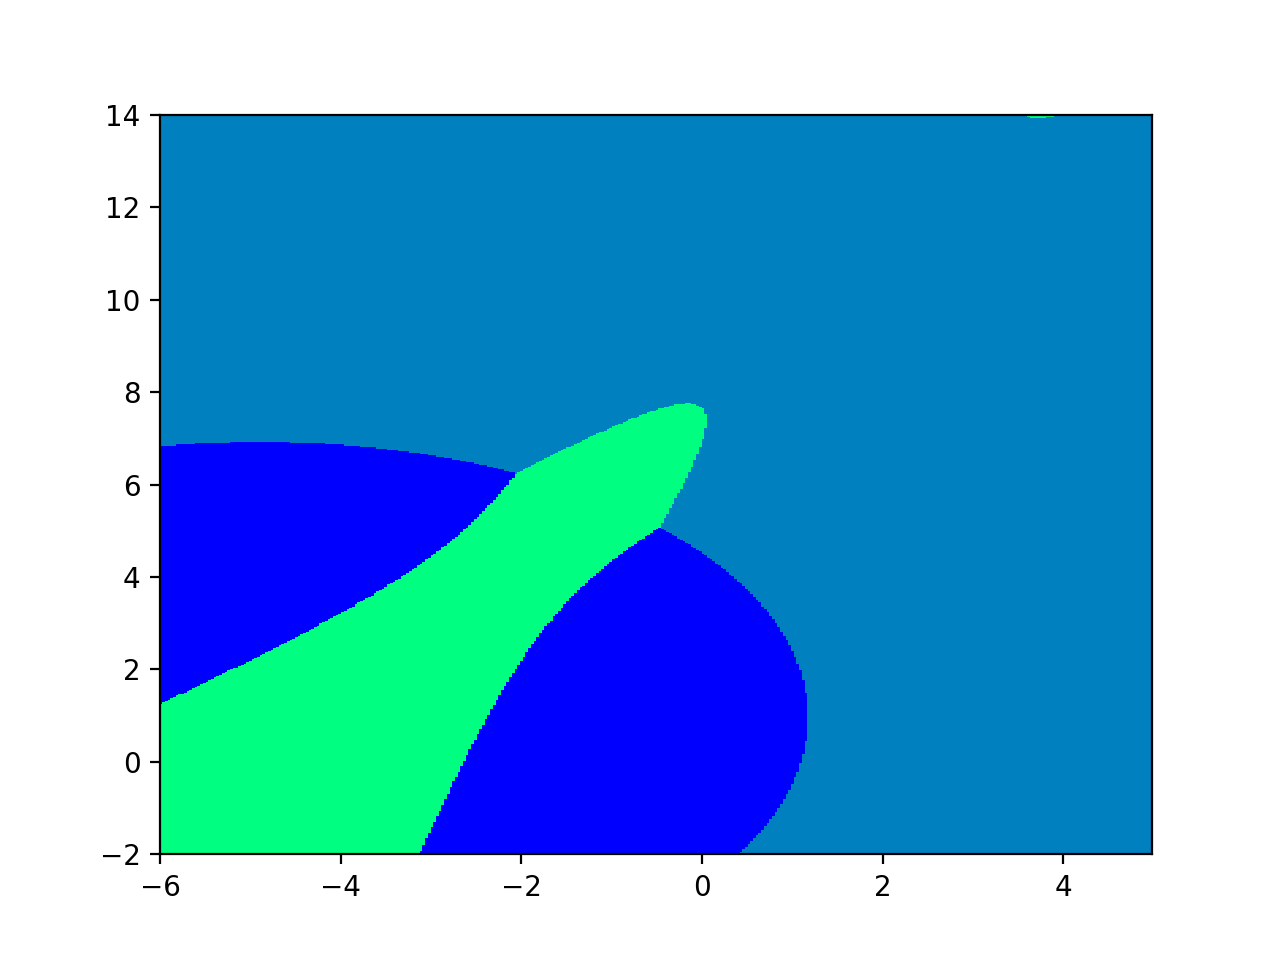
\includegraphics[width=0.6\linewidth]{decision_boundaries}
	\caption{Generated decision boundaries}
	\label{fig:decision_boundaries}
\end{figure}

\part{c} (10 pts) Calculate test accuracy and write it into the report.

\tab \textbf{Accuracy:} 0.79

\question{2}{Logistic Regression}

\part{a} (25 pts) Calculate accuracy and confusion matrix using 10 fold cross validation and write them into the report. Which classes are most confused with each other?

\begin{table}[h]
	\centering
	\caption{Accuracy confussion matrix when Learning rate: 0.01, Iteration Count: 250,}
	\label{my-label}
	\begin{tabular}{|c|c|c|c|}
		\hline
		& Iris-setosa (Predicted) & Iris-versicolor (Predicted) & Iris-virginica (Predicted) \\ \hline
		Iris-setosa (Actual)     & 50                      & 0                           & 0                          \\ \hline
		Iris-versicolor (Actual) & 0                       & 46                          & 4                          \\ \hline
		Iris-virginica (Actual)  & 0                       & 5                           & 45                         \\ \hline
	\end{tabular}
\end{table}

Iris-versicolor and Iris-virginica are most confused with each other.

\part{b} (25 pts) Analyze the effect of learning rate(η). Use 10 fold cross validation and compare your results with different learning rates are 10, 1, 0.1, 0.01 based on the number of iterations and classification accuracy.

\begin{eqnarray*}
\text{Learning rate: 0.01}, & \text{Iteration Count: 250},& \text{Accuracy: 0.9466666666666689} \\
\text{Learning rate: 0.1}, &\text{Iteration Count: 250},& \text{Accuracy: 0.9400000000000022} \\
\text{Learning rate: 1}, &\text{Iteration Count: 250},& \text{Accuracy: 0.9466666666666689} \\
\text{Learning rate: 10}, &\text{Iteration Count: 250},& \text{Accuracy: 0.9533333333333356} \\
\end{eqnarray*}

According to the results, the accuracy of logistic regression is non-linear for learning rates.

\end{document}
